\documentclass{beamer}
\usepackage[utf8]{inputenc}
\usepackage{../UnipdTheme/Padova/beamerthemePadova}
\usepackage[absolute,overlay]{textpos}
\usepackage{graphicx}

\title{Layout delle tastiere}
\subtitle{Come inserire gli accenti in laboratorio}
\author{Davide Polonio, Marco Zanella \& Emanuele Carraro}
\date{AA 2017-2018}

\begin{document}

	\maketitle
    \begin{frame}{Gli accenti nelle tastiere}

Se guardate le tastiere in laboratorio noterete che sono differenti da quelle
che avete a casa

\vfill

Sono tastiere con layout americano che vanno molto bene per scrivere codice
e in lingua inglese ma molto meno per scrivere in italiano

\vfill

Il problema vero è che non vedete gli accenti

\end{frame}

    \begin{frame}{Cambiare il layout della tastiera - 1}

\begin{figure}
\centering
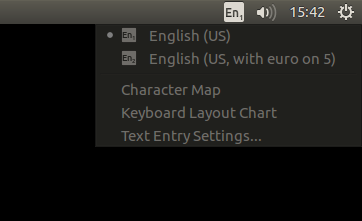
\includegraphics[scale=0.8]{res/img/1}
\end{figure}

\end{frame}
    \begin{frame}{Cambiare il layout della tastiera - 2}

\begin{figure}
\centering
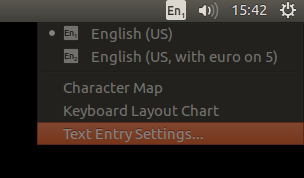
\includegraphics[scale=0.9]{res/img/2}
\end{figure}

\end{frame}
    \begin{frame}{Cambiare il layout della tastiera - 3}

\begin{figure}
\centering
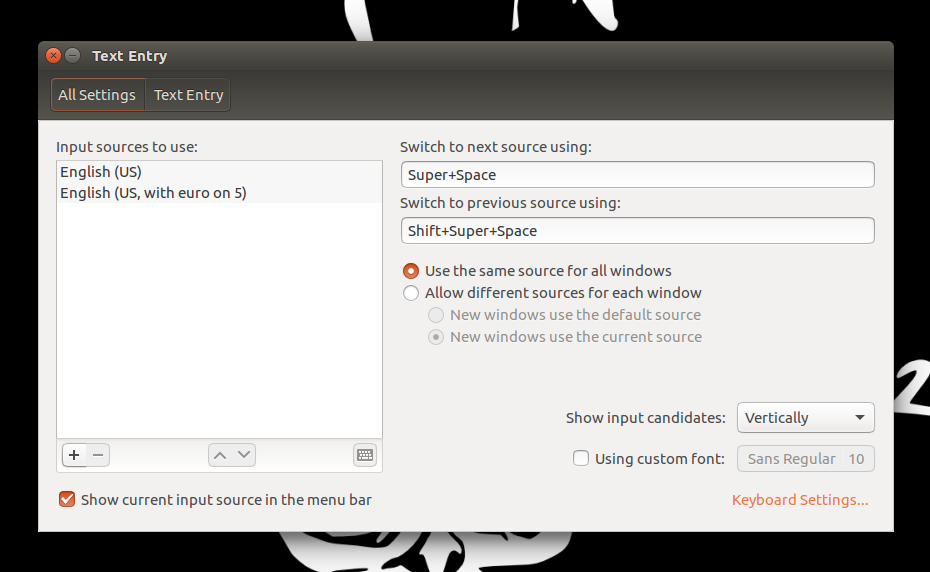
\includegraphics[scale=0.31]{res/img/3}
\end{figure}

\end{frame}
    \begin{frame}{Cambiare il layout della tastiera - 4}

\begin{figure}
\centering
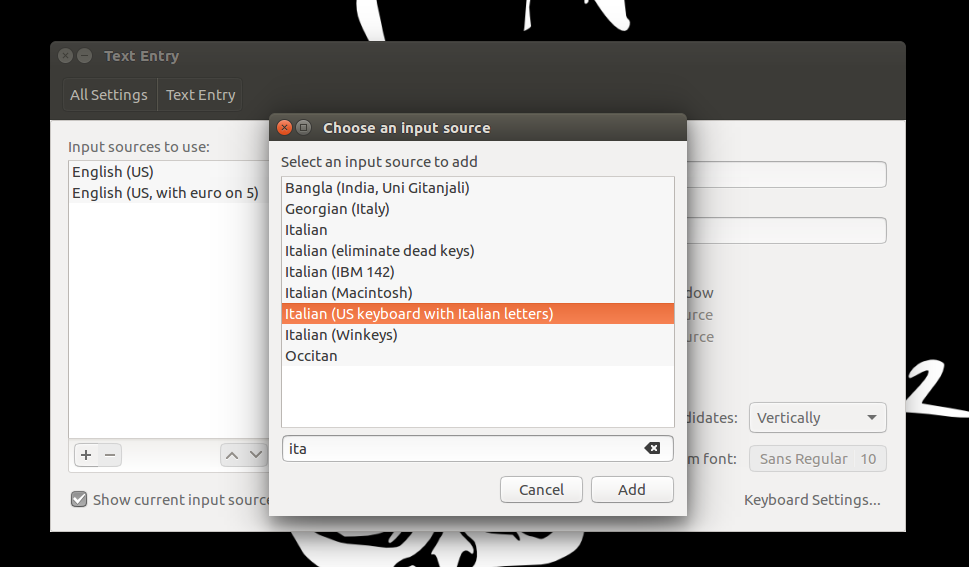
\includegraphics[scale=0.31]{res/img/4}
\end{figure}

\end{frame}
    \begin{frame}{Cambiare il layout della tastiera - 5}

\begin{figure}
\centering
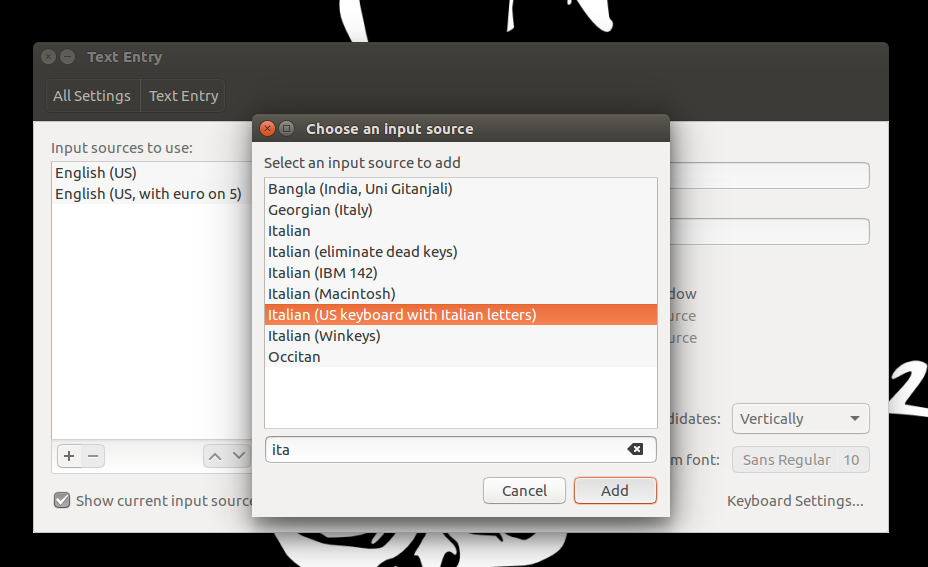
\includegraphics[scale=0.31]{res/img/5}
\end{figure}

\end{frame}
    \begin{frame}{Cambiare il layout della tastiera - 6}

\begin{figure}
\centering
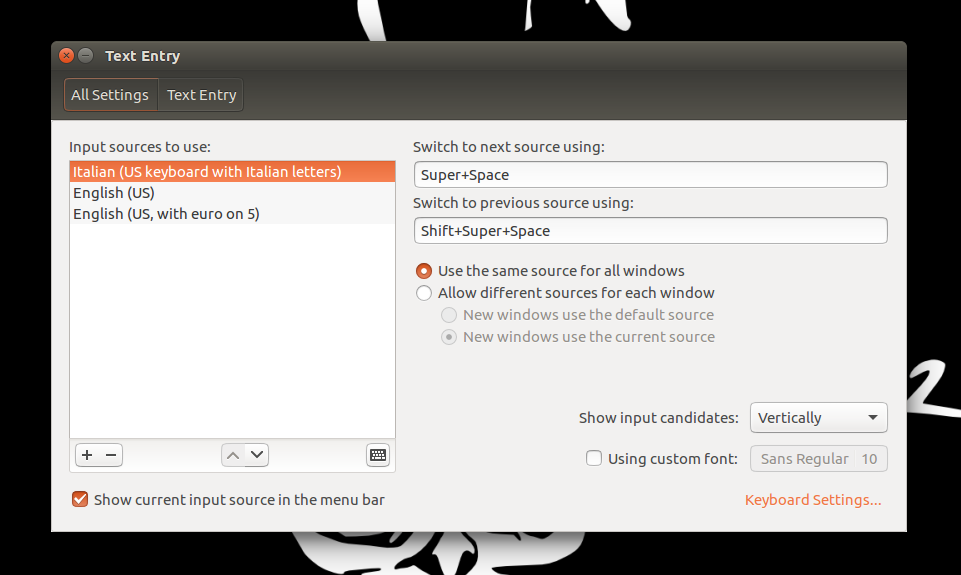
\includegraphics[scale=0.31]{res/img/6}
\end{figure}

\end{frame}
    \begin{frame}{Cambiare il layout della tastiera - 7}

\begin{figure}
\centering
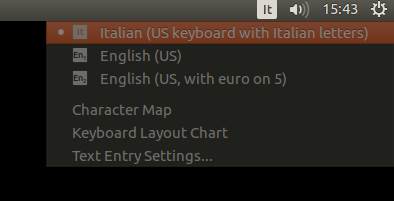
\includegraphics[scale=0.75]{res/img/7}
\end{figure}

\end{frame}
    \begin{frame}{Inserimento di una lettera accentata}

\vfill
\centerline{\textbf{\Huge{Alt Gr + lettera}}}
\vfill

\end{frame}

\end{document}